%!TEX root = ../../../root.tex

\paragraph{Manifold hypothesis}

How can such a mapping produce samples that resemble the observed data? It must be that there is some lower-dimensional structure (\emph{manifold}) on which the data are constrained, and this structure is \emph{embedded} in the higher-dimensional space. 

Imagine text on a piece of paper: it naturally lives in the plane. However, if the paper is folded, we do not have a plane any longer, so we must represent this text in the 3D space. Nonetheless the text cannot leave the paper, it is constrained to lie onto it, but the paper (structure) is now \emph{curved} and must be described (\emph{embedded}) in a higher-dimensional space.

The decoder performs a mapping from a low-dimensional \emph{latent space} to a high-dimensional \emph{embedding space}. When we train an autoencoder we are learning a parametric model of a latent space, i.e. the underlying, lower-dimensional structure of the data.

We have already seen this concept: the \emph{manifold hypothesis}. Given some data, e.g. images of the Eiffel tower, we can represent the data as set of points $\vb{x}$ in some high-dimensional space; however, the manifold hypothesis states that the way they are positioned in this high-dimensional space will not be random, but will have a \emph{structure}, forming a ``hyper-surface'', or more precisely, a \emph{manifold}. This structure encodes some information that all the datapoints have in common, therefore not every component of the points $\vb{x}$ are independent, but instead there are constraints that ensure that the points stay on the structure. The datapoints have \emph{fewer degrees of freedom} than the dimensionality of the space.

If we know the \emph{geometry} of such structure, i.e. if we know these constraints, we can drop all the components whose value will be determined by other components and constraints, i.e. we can describe the different datapoints in a much smaller-dimensional space. However, the structure is in general \emph{not} an Euclidean space (unless the structure is trivially an hyper-plane), but instead a \emph{surface}, more in general a curved space or formally a \emph{manifold}. Recall that we defined vector spaces in the Euclidean domain, so in general we cannot represent datapoints in the embedding space as vectors, and also keep the underlying structure: the sum of two vectors representing datapoints lying on the manifold will be a vector that does not lie on the manifold, just like naively summing two images of the Eiffel tower will not result in an image of the Eiffel tower.

\paragraph{Manifolds}

How can we deal with manifolds, but still keep the Euclidean formalism that was so useful to us? 

Formally, an $n$-dimensional manifold, or $n$-manifold for short, is a \emph{topological space} (a space with the additional concept of \emph{neighborhood}) with the property that each point is \emph{locally homeomorphic} to Euclidean space $\mathbb{R}^n$. 

``Locally homeomorphic to Euclidean space'' means that every point has a \emph{neighborhood} homeomorphic to a neighborhood in Euclidean space, that is simply a $n$-ball, i.e. an hypersphere of a certain radius $\delta$. 
Two neighborhoods are ``homeomorphic'' if there exists a \emph{homeomorphism} between them, i.e. a smooth and invertible mapping from the points of the first to the points of the second. Notice that this means that points that are ``close'' on the manifold must be ``close'' also on the corresponding Euclidean space.

Informally, this means that at each point on the manifold, that is a curved space, we can locally think to lie on a \emph{flat}, Euclidean space instead. The more we zoom out from the point, the more this approximation loses accuracy, but this is enough for us to define \emph{locally} a Euclidean vector space. For instance, we live on the surface of Earth, a curved space, but locally we have the illusion of living on a flat space, so Euclidean distance makes sense to us, even though it is not globally correct (and in fact this must be accounted for when charting intercontinental courses, e.g. to go from $A$ to $B$ it may be shorter to go north from $A$ to $C$ and then south again to $B$ instead of going straight from $A$ to $B$).

In the following we will refer to curves and surfaces, as manifolds embedded in $\mathbb{R}^3$, since they are easier to visualize.

\paragraph{Differential geometry}

The study of local properties of curves and surfaces is the realm of \emph{differential geometry}. The overall idea is that we can model mathematically a surface as a collection of neighborhoods (colored regions in \cref{fig:bunny}) and we require that the union of these regions should cover the entire surface and that each region can be mapped in a well-behaved way to a subset of $\mathbb{R}^2$ (Note that if we have a high dimensional surface the subset would be in some other dimension not necessarily two).
\begin{figure}[H]
	\centering
	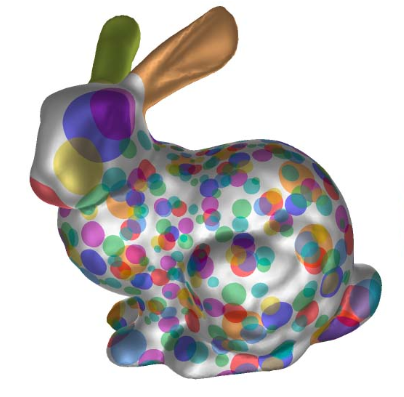
\includegraphics[width=.5\textwidth]{11/bunny_local}
	\caption{An example of differential geometry.}\label{fig:bunny}	
\end{figure}
A differentiable manifold can be described using these maps, called coordinate \emph{charts}. It is not generally possible to describe a manifold with just one chart, because the global structure of the manifold is different from the simple (Euclidean) structure of the charts. For example, no single flat map can represent the entire Earth without separation of adjacent features across the map's boundaries (although Russia and Alaska are adjacent, they appear separated on the map). Instead, we need several charts, collected in what is called an \emph{atlas}.
\begin{figure}[H]
	\centering
	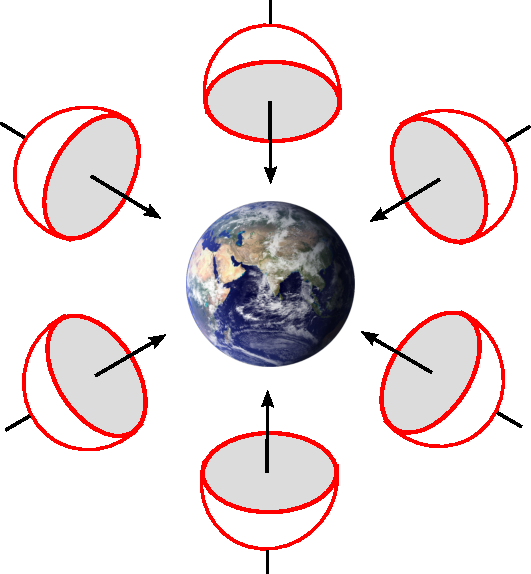
\includegraphics[width=.4\textwidth]{11/charts}
	\caption{An atlas of e.g. $6$ charts is able to correctly represent Earth. Notice two would suffice, but in general the minimum number is not trivial to compute.}\label{fig:sphere}	
\end{figure}
Formally, a chart is a map 
\begin{equation}
    \phi: \mathbb{R}^2 \to \mathcal{S} \subset \mathbb{R}^3
\end{equation} 
with the property of being
\begin{itemize}
    \item invertible (we can go from a point on the surface to one in the plane and back);
    \item continuous (closeby points must be mapped by $\phi$ to closeby points).
\end{itemize}
If such mapping is also differentiable then we say that $\phi$ is a \emph{diffeomorphism}; if it is infinitely-differentiable it is also said to be \emph{smooth}.
\begin{figure}[H]
	\centering
	\begin{overpic}
		[trim=0cm 0cm 0cm 0cm,clip,width=0.35\linewidth]{11/charts_2.pdf}
		\end{overpic}\hspace{1.5cm}
		\begin{overpic}
		[trim=0cm 0cm 0cm 0cm,clip,width=0.32\linewidth]{11/map.png}
		\put(38,-11){\footnotesize chart}
		\end{overpic}
	\caption{Chart representation.}\label{fig:chart}	
\end{figure}

General manifolds can be $k$-dimensional, meaning that we have charts:
\begin{equation}
	\phi: \mathbb{R}^k \to \mathcal{M} \subset \mathbb{R}^d \quad \text{with } k < d.
\end{equation}
Note that the choice of $\phi$ and the choice of the subset of the euclidean space is not unique.

\paragraph{Decoders as a chart}

The decoder of an autoencoder learns a mapping 
\begin{equation}
    D: \mathbb{R}^k \to \mathbb{R}^d
\end{equation}
from a low-dimensional Euclidean space, the latent space $\mathbb{R}^k$ spanned by the codes $\vb{z}$, to a higher-dimensional embedding space, the data space $\mathbb{R}^d$ spanned by the observed datapoints $\vb{x}$. 

Such a mapping is differentiable, since it is defined by a neural network, and (in principle) is invertible via encoder $E$. Therefore, under the manifold hypothesis, the destination space is actually a manifold $\mathcal{M}$ and the mapping that the decoder is learning is a valid (parametric, via the network weights) chart for the manifold.
\begin{equation}
    D: \mathbb{R}^k \to \mathcal{M} \subset \mathbb{R}^d
\end{equation}

However, we do not know in advance the dimension of $\mathcal{M}$, i.e. the dimension of the Euclidean space $\mathbb{R}^k$ to which it is locally homeomorphic, therefore when designing autoencoders one should employ a trial and error strategy to decide the dimension $k$ of the latent space, and see which choice yields the best results.
